\documentclass[dvipdfmx]{jsarticle}

\title{JavaScript入門その1}
\author{原著者:清水健二 / 改訂:糠山誠一}
\date{2020-06-13}
\usepackage{tcolorbox}
\usepackage{color}
\usepackage{listings, plistings}

% Java
\lstset{% 
  frame=single,
  backgroundcolor={\color[gray]{.9}},
  stringstyle={\ttfamily \color[rgb]{0,0,1}},
  commentstyle={\itshape \color[cmyk]{1,0,1,0}},
  identifierstyle={\ttfamily}, 
  keywordstyle={\ttfamily \color[cmyk]{0,1,0,0}},
  basicstyle={\ttfamily},
  breaklines=true,
  xleftmargin=0zw,
  xrightmargin=0zw,
  framerule=.2pt,
  columns=[l]{fullflexible},
  numbers=left,
  stepnumber=1,
  numberstyle={\scriptsize},
  numbersep=1em,
  language={Java},
  lineskip=-0.5zw,
  morecomment={[s][{\color[cmyk]{1,0,0,0}}]{/**}{*/}},
}
%\usepackage[dvipdfmx]{graphicx}
\usepackage{url}
\usepackage[dvipdfmx]{hyperref}
\usepackage{amsmath, amssymb}
\usepackage{itembkbx}
\usepackage{eclbkbox}	% required for `\breakbox' (yatex added)
\fboxrule=0.5pt
\parindent=1em
\begin{document}

%% 修正時刻: Sat Jun 13 16:00:25 2020


\section{HTMLに直接JavaScriptを書く}

\subsection{JavaScript構文}

\subsubsection{window.alert();}

start.html の \verb!<script>...</script>!内にJavaScriptを記述することができます。\\
\fbox{window.alert('伝えたい内容');} でアラートウィンドウを表示できます。\\
ブラウザの更新ボタンをクリックして確認してください。

\begin{lstlisting}
 <script>
   window.alert(100);
 </script>
\end{lstlisting}

数字の場合はそのままでかまいませんが、文字の場合は必ず ``''(ダブルクォーテーション)
もしくは ''(シングルクォーテーション)で囲んでください。\\

''100'' のかわりに文字を入れてみます。

\begin{lstlisting}
 <script>
   window.alert('こんにちは');
 </script>
\end{lstlisting}

\subsubsection{関数を書いて実行する}

\fbox{function 関数名 () \{ 処理 \} } で、関数内に複数の構文を書くことができます。\\
関数は複数の処理をまとめるのに便利です。「メソッド」と呼ばれる場合もあります。

\begin{lstlisting}
 <script>
   function kansu1 () {
     window.alert(100);
   }
 </script>
\end{lstlisting}

このままでは中の alert は実行されません。関数を実行するためには関数以外の場所で
\fbox{関数名();} を記述して実行する必要があります。

\begin{lstlisting}
 <script>
   function kansu1 () {
     window.alert(100);
   }
   // 下記を追加。
   kansu1();
 </script>
\end{lstlisting}

\subsubsection{onclick=''関数名()``で実行}

関数を使うことで処理を特定のタイミングで実行することができるようになります。\\
例えば「ボタン」を押したときに関数の内容を実行させることができます。\\
start.html の \verb!<body>! 内の \verb!<button>! タグに \\
\hspace{5mm} \verb!<button onclick="kansu1()">! \\
と記述してあることに注意してください。\\
ブラウザのボタンをクリックしてアラートが表示されたら成功です。

\subsection{変数}

  \subsubsection{変数を設定する}

JavaScriptでは、''変数''と言われる入れ物の中に好きな文字や数字等を入れることができます。\\
ここでは、新しい関数 ''kansu2''の中に変数を入れてその内容を表示します。\\
変数の設定には、以前は \fbox{ var 変数名; } とすることが多かったのですが、最近は
\fbox{ const 変数名; } や \fbox{ let 変数名; } が主流です。

 \begin{tcolorbox}
  \begin{itemize}
   \item \textbf{const} -- 一度文字や数字を入れたら、再代入できない。
   \item \textbf{let}   -- 再代入できる。
  \end{itemize}
 \end{tcolorbox}

たいていは再代入する必要がないので、\textgt{const}をよく使います。再代入の必要があるときは、
\textgt{let}を使います。

代入のために、''\textbf{=}''を使います。
数学で使ったのとは意味が違うので、注意してください。

\begin{lstlisting}
 <script>
   function kansu2 () {
     // 変数を設定
     const hensu = 200;
     // 変数の内容を実行
     window.alert(hensu);
   }
 </script>
\end{lstlisting}

\subsubsection{見出しをonclickして関数を実行する}

\fbox{kansu2();} も何処かでクリックしないと内容が表示されません。\\
ここでは \verb!<h1>!タグをクリックしたときに実行されるように修正します。

\textbf{start.html} の \verb!<h1>!タグの部分を下記のように変更してください。

\begin{verbatim}
    <h1 id="heading1" onclick="kansu2()">ここは見出しですがボタンにもできます</h1>
\end{verbatim}

アラートに変数の内容が表示されればOKです。

onclick=''''属性は、ボタン以外にもHTMLタグの中ならばどこにでも書けます。


   \subsubsection{
   \textless body \textgreater タグの内部に
   \textless script \textgreater タグを書いて実行}

\verb!<script>...</script>! と JavaScript は、\verb!<head>!内に書くほかに、
\verb!<body>! タグ内に書いても問題ありません。

\begin{lstlisting}
 <ul>
   <li>HTMLで書きました</li>
   <!-- JSはbody内にも書ける -->
   <script>

   </script>
 </ul>
\end{lstlisting}

\subsubsection{document.write}

HTMLタグ(ここでは \verb!<li>! タグ)を、アラートではなく直接文字として表示します。

HTML上にテキストを表示させるには document.write が便利です。

\begin{lstlisting}
 <ul>
   <li>HTMLで書きました</li>
   <!-- JSはbody内にも書ける -->
   <script>
     document.write("JS");
   </script>
 </ul>
\end{lstlisting}

document.writeはHTMLタグも記述できます。

\begin{lstlisting}
 <ul>
   <li>HTMLで書きました</li>
   <!-- JSはbody内にも書ける -->
   <script>
     document.write('<li>JS</li>');
   </script>
 </ul>
\end{lstlisting}

\subsubsection{変数と文字の結合}

変数の内容や文字は ``+''演算子で結合できます。

\begin{lstlisting}
 <ul>
   <li>HTMLで書きました</li>
   <!-- JSはbody内にも書ける -->
   <script>
     const listText = 'JS';
     document.write('<li>' + listText + '</li>');
   </script>
 </ul>
\end{lstlisting}

\subsubsection{テンプレート文字列で変数の内容を表示(ES2015)}

ES2015 からは、document.write() の中身を `バッククォート(shiftキー + @) ではさむことで
スマートに変数を表示できるようになりました。バッククォート内で展開される変数を
''\textbf{テンプレート変数}'' と呼びます。テンプレート変数を展開するには
 \textbf{\$\{変数名\}} と記述します。

\begin{lstlisting}
 <ul>
   <li>HTMLで書きました</li>
   <!-- JSはbody内にも書ける -->
   <script>
     const listText = 'ES2015';
     document.write(`<li>${listText}</li>`);
   </script>
 </ul>
\end{lstlisting}

\subsection{条件分岐}

再度、\verb!<head>!タグ内の \verb!<script>...</script>! に戻ります。

\begin{lstlisting}
 <script>
   function kansu2 () {
     // 変数を設定
     const hensu = 200;
     // 変数の内容を実行
     window.alert(hensu);
   }
 </script>
\end{lstlisting}

\subsubsection{IF(条件式) \{...\} else \{...\}}

下記のように書くことで条件別でアラートの内容を変更できます。

\begin{lstlisting}
 <script>
   const hensu = 100;
   // if文
   if (hensu >= 70) {
     window.alert('OK');
   }
 </script>
\end{lstlisting}

hensu の内容が 70以上なので、アラートにOKが表示されます。

また、次のように条件を満さなかった場合も記述することもできます。

\begin{lstlisting}
 <script>
   const hensu = 50;
   // if文
   if (hensu >= 70) {
     window.alert('OK');
   } else {
     window.alert('NG');
   }
 </script>
\end{lstlisting}

今回は hensu の値を 50 にしたので、アラートに NG と表示されました。

\subsubsection{関数に IF文を書いてボタンで実行する}

関数内に if文を書くことで好きなタイミングで条件式を実行できます。

\begin{lstlisting}
 <script>
   // 関数名を kansu2 から kausu1 に変更する。
   funcsion kansu1 () {
     const hensu = 100;

     if (hensu >= 70) {
       window.alert('Ok');
     } else {
       window.alert('NG');
     }
   }
 </script>
\end{lstlisting}

ボタンには \fbox{onclick=''kansu1()''} が設定されているので、クリックす
ることでアラートを表示できるはずです。


\subsubsection{IF文で背景色を変える}

JavaScriptにはCSSと同じ効果を持つ構文があります。先ほどのIF文を次のように変更してください。

\begin{lstlisting}
 <script>
   // 関数名を kansu2 から kausu1 に変更する。
   funcsion kansu1 () {
     const hensu = 100;

     if (hensu >= 70) {
       document.body.style.backgroundColor = 'red';
     } else {
       document.body.style.backgroundColor = 'yellow';
     }
   }
 </script>
\end{lstlisting}

ページの背景色が変更されれば成功です。

\subsection{反復処理}

先ほどの \verb!<ul>...</ul>! 内に書いたスクリプトに戻ります。

\begin{lstlisting}
 <ul>
   <li>HTMLで書きました</li>
   <script>
     const listText = 'ES2015';
     document.write(`<li>${listText}</li>`);
   </script>
 </ul>
\end{lstlisting}

   \subsubsection{FOR文}

今までは const を使いましたが、今度は let を使います。再代入を行うからで
す。

\begin{lstlisting}
 <ul>
   <li>HTMLで書きました</li>
   <script>
     const listText = 'ES2015';

     for (let i = 0; i < 5; i++) {
       document.write(`<li>${listText}</li>`);
     }
   </script>
 </ul>
\end{lstlisting}

\fbox{for ( ... )} の中で繰り返しのための条件を記述しています。

まず、\fbox{let i = 0;} で、変数i を設定し、0という初期値を代入します。

次の \fbox{i \textless \ 5} で、終了条件いいかえると繰り返し条件を記述しています。i が 5 未満である間は処理を行うということです。

3つめの \fbox{i++} は、プログラミング独特の記述法で、i に i+1 を代入する
\fbox{i = i + 1} を短く記述したものです。要するに i を1増やすということです。

つまり、i が 0 から 4 までの間、5回処理を繰り返すという意味です。

\fbox{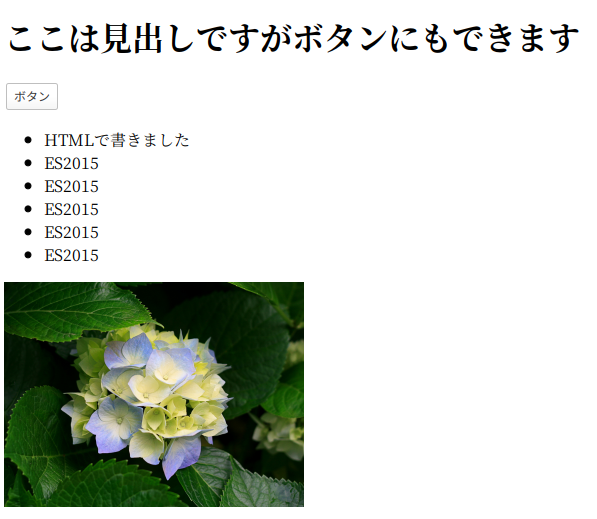
\includegraphics[width=10cm]{kurikaesi.png}}


\subsubsection{FOR文を使って番号を振る}

for文内で使われている変数 i は 0...5 の数字を持っています。
これを document.write に記述することで、連番リストを作ることができます。
コードを以下のように変更してください。

\begin{lstlisting}
 <ul>
   <li>HTMLで書きました</li>
   <script>
     const listText = '';

     for (let i = 0; i < 5; i++) {
       listText = 'list' + i;
       document.write(`<li>${listText}</li>`);
     }
   </script>
 </ul>
\end{lstlisting}

うまく表示できたでしょうか? たぶん表示しなかったはずです。
原因を調べて みましょう。


ブラウザ上で右クリックをして ``検証''を選択してください。
すると、デベロッパーツールが起動します。そして、赤い×の印が
でているはずです。

``console'' を選択すると、エラーメッセージが表示されています。
そして、そこには

\fbox{TypeError: Attempted to assign to readonly property.}

というような内容が表示されているはずです。これは、

\fbox{タイプエラー:読み取り専用プロパティに割当てようとしました}

という意味です。

そして、行番号も表示されているはずです。

\fbox{ listText = 'list' + i;} の行です。

このエラーは、const に再代入をしようとしたから起こったのです。

consgt を let に書き換えてください。それからブラウザを再読込してください。

\begin{lstlisting}
 <ul>
   <li>HTMLで書きました</li>
   <script>
     let listText = '';

     for (let i = 0; i < 5; i++) {
       listText = 'list' + i;
       document.write(`<li>${listText}</li>`);
     }
   </script>
 </ul>
\end{lstlisting}

\fbox{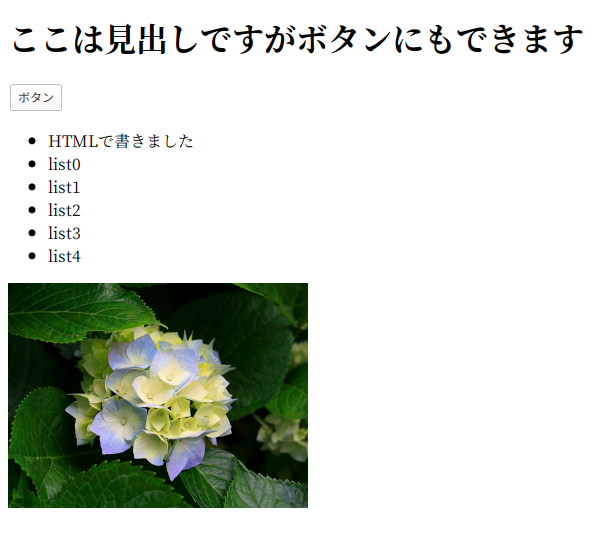
\includegraphics[width=10cm]{list0-5.png}}

\subsection{document.write() は非推奨}

\begin{tcolorbox}[title=document.write() は非推奨]
さて、今までブラウザの画面に文字を書き出したり、\verb!<li>!などのタグを出力したりするのに
document.write() を使ってきましたが、実はこのメソッドは \textbf{非推奨} だったのです!

 \begin{thebibliography}{9}
  \bibitem{document_write} HTML Living Standard - document.write() \\
          \url{https://html.spec.whatwg.org/multipage/dynamic-markup-insertion.html#document.write()}
  \bibitem{Document.write} Document.write() - MDN \\
          \url{https://developer.mozilla.org/ja/docs/Web/API/Document/write}
 \end{thebibliography}

 グーグル翻訳ではよくわからないのですが、どうもブラウザの動作に悪い影響を与え、想定外の描写になる
 可能性があるようで、代りに innerHTMLメソッド、insertAdjacentHTMLメソッド、textContentメソッドを
 使うとよいということです。\\
 \verb!<li>!などのタグも含めて文字列を挿入するなら、innerHTMLが簡単です。\\
 また、単に文字列だけなら、textContentでいいと思います。\\
 insertAdjacentHtmlはタグの挿入位置も含めて指定できます。大変強力です。 \\
 これらのメソッドは、後ほど紹介します。
\end{tcolorbox}

\subsection{SWITCH文}

次の作業は、\verb!<head>!内の \verb!<script>!文で行います。

\begin{lstlisting}
 <script>
   const hensu = 100;

   if (hensu >= 70) {
     document.body.style.backgroundColor = 'red';
   } else {
     document.body.style.backgroundColor = 'yellow';
   }
 </script>
\end{lstlisting}

\verb!<script>...</script>!内を書き換えます。

\begin{lstlisting}
 <script>
   const hensu = 0;
   let result = '';

   switch (hensu) {
     case 0:
       result = '大吉';
       break;
     case 1:
       result = '中吉';
       break;
     case 2:
       result = '小吉';
       break;
     case 3:
       result = '末吉';
       break;
     default:
       result = '吉';
    }

   window.alert(result);
 </script>
\end{lstlisting}

これを関数 kansu2() とします。

\begin{lstlisting}
 <script>
   function kansu2 () {
 
     const hensu = 0;
     let result = '';

     switch (hensu) {
       case 0:
         result = '大吉';
         break;
       case 1:
         result = '中吉';
         break;
       case 2:
         result = '小吉';
         break;
       case 3:
         result = '末吉';
         break;
       default:
         result = '吉';
      }
  
     window.alert(result);
   }
   </script>
\end{lstlisting}

\verb!<h1>! は onclick属性で kansu2() を指定しているので、ブラウザで表示
させたら \verb!<h1>!部分をクリックすると ''大吉'' と表示されます。

\subsubsection{乱数を使う}

さて、この kansu2()は、\fbox{ const hensu = 0; } としているので、常に大吉が表示されます。

これを御神籤らしくするために、''乱数''というメソッドを使います。

JavaScriptにはさまざまなオブジェクトが備わっているのですが、そのうちの一つに ''Math'' と
いうオブジェクトがあります。これは数学で使うものが集められています。

Math.random() とすると、0から1未満 の間の数値をランダムに得ることができます。(0.1 ... 0.9)

Math.random() * 5 とすると、0から5未満の間の数値をランダムに得られます。(0.1 ... 4.9)

kansu2 を記述していた箇所に以下のように書き加えてください。

\begin{lstlisting}
 <script>
   function kansu2 () {

     console.log( Math.random() * 5);    // <-- これ
 
     const hensu = 0;
     let result = '';

     switch (hensu) {
       case 0:
         result = '大吉';
         break;
       case 1:
         result = '中吉';
         break;
       case 2:
         result = '小吉';
         break;
       case 3:
         result = '末吉';
         break;
       default:
         result = '吉';
      }
  
     window.alert(result);
   }
   </script>
\end{lstlisting}

ブラウザで再読込したあと、デベロッパーツールを開いて、''console''を表示しておいてください。\\
それから \verb!<h1>! 部分をクリックすると、''console''にその時生成された乱数が表示される
はずです。クリックするたびに数値が変化するのがわかります。\\

次に、乱数を小数値ではなく、整数にします。これは、小数点以下を切り捨ててみます。\\
乱数を生成している部分を以下のようにしてください。

\fbox{ console.log( Math.floor( Math.random() * 5 )); }

小数値が整数に変ったのが確認できます。これで、準備が整いました。\verb!<script>...</script>!
の中を以下のようにしてください。

\begin{lstlisting}
 <script>
   function kansu2 () {
     const hensu = Math.floor( Math.random() * 5 );
     console.log('hensu:', hensu);
 
     let result = '';

     switch (hensu) {
       case 0:
         result = '大吉';
         break;
       case 1:
         result = '中吉';
         break;
       case 2:
         result = '小吉';
         break;
       case 3:
         result = '末吉';
         break;
       default:
         result = '吉';
      }
  
     window.alert(result);
   }
   </script>
\end{lstlisting}

\fbox{ console.log() } は、プログラム中の変数の値がどうなっているのかを調べるのに重宝します。
ここでは、
\begin{verbatim}
    console.log('hensu:', hensu);
\end{verbatim}
としましたが、
\begin{verbatim}
    console.log('hensu:' + hensu);
\end{verbatim}
とすることも可能です。


\end{document}

%% 修正時刻: Sat May  2 15:10:04 2020


%% 修正時刻: Sun Jun 14 20:05:13 2020
